\documentclass{article}
\usepackage{tikz}
\usetikzlibrary{shapes, arrows, positioning, fit, backgrounds}


% Define block styles
\tikzstyle{decision} = [diamond, draw, fill=yellow!40, 
    text width=4.5em, text badly centered, node distance=1.75cm, inner sep=0pt]
\tikzstyle{decisiong} = [diamond, draw, fill=blue!40, 
    text width=4.5em, text badly centered, node distance=1.75cm, inner sep=0pt]
\tikzstyle{block} = [rectangle, node distance=1.75cm, minimum width=1cm, minimum height=0.5cm, draw, fill=yellow!20, 
    text width=20em, text centered, rounded corners, minimum height=1.5em]
\tikzstyle{blockg} = [rectangle, minimum width=0.5cm, minimum height=0.5cm, draw, fill=violet!40, 
    text width=15em, text centered, rounded corners, minimum height=1.5em]
\tikzstyle{line} = [draw, -latex']
\tikzstyle{cloud} = [draw, ellipse,fill=yellow!20, node distance=1.5cm, 
    minimum height=2em]
\tikzstyle{invis} = [draw, fill=yellow!10, node distance=4.25cm, 
    minimum height=2em]
\tikzstyle{invisg} = [draw, fill=yellow!10, node distance=3.5cm, 
    minimum height=2em]
\tikzstyle{matheq} = [node distance=8.75cm, text width=21em, minimum width=1cm, 
    minimum height=2em, text centered]


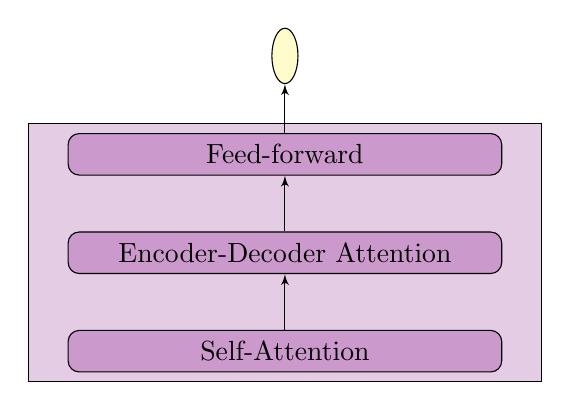
\begin{tikzpicture}[node distance = 1.25cm, auto]
    % Place nodes
    \node [cloud] (init) {};

    \node [blockg, below of=init] (third) {Feed-forward};
    \node [blockg, below of=third] (fourth) {Encoder-Decoder Attention };
    \node [blockg, below of=fourth] (fifth) {Self-Attention };

 

    \begin{scope}[on background layer]
    \node[draw, fill=violet!20, fit=(third) (fifth), inner xsep=5mm]{};
    \end{scope}
    % Draw edges
    \path [line] (third) -- (init);
    \path [line] (fourth) -- (third);
    \path [line] (fifth) -- (fourth);


\end{tikzpicture}
